\subsection{Gene analysis} \label{s:lit:gene_analysis}


% Introduce the methods
Throughout the project there are different methods on finding the \acrfull{mibc} subgroups using the network approach followed then by the clustering analysis (\cref{s:N_I,s:N_II}) or by just applying different clustering models as in \cref{s:clustering_analysis}. In both cases there are new subgroups that need to be biologically interpret with the goal to both biologically validate as well as to find new marker or new functions. To achieve this there are three methods used: \acrfull{dea}, pi-plots and \acrfull{gsea} which are covered in the following subsections. 

% Highlight the flow
% Who introduced the method
The \acrshort{dea} is the most important tool as it allows to determine the genes that are specific to a subtype compare to the other. The values derived using the method are used to create the Volcano plots, see \cref{s:lit:dea}, allowing statistical analysis of the gene expression between two groups. The results of the \acrshort{dea} can also be used to compute the pi-values \citet{Xiao2014-zn} which allows the comparison of four groups in one plot; see \cref{s:lit:pi}. Subsequently, the pi-value plots can be used to compute ranking for specific groups which can be used to perform \acrlong{gsea}; see \cref{s:lit:gsea}.


% DEA
\subsubsection{Volcano plot} \label{s:lit:dea}


% Intro to the volcano plot
The project employed the sleuth method introduced by \citet{Pimentel2017-xp} for differential analysis of the RNAseq data. This method takes as input a file containing the samples, their cluster labels, and the paths to the raw RNAseq reads. It returns the \textit{q} and \textit{p} values for each gene, indicating the significance of the expression differences.

% How the Volcano figure is constructed
The $-log_{10}$ transformed \textit{p}-values constitute the Y-axis in a volcano plot, while the X-axis displays the $log_{2}$ transformed fold-change in gene expression between the two groups. This means that the volcano plot, as shown in \cref{fig:lit:dea_eg}, displays the magnitude of gene expression change on the horizontal axis and the significance of that change on the vertical axis.

% Interpretation
In \cref{fig:lit:dea_eg}, two sides of the plot represent the two compared subgroups: "Abs-Ca large" and "Abs-Ca small." The further up a gene is on the left side, the more differentially expressed it is in the "Abs-Ca large" group; conversely, genes in the right corner are more differentially expressed in the "Abs-Ca small" group. The scale of the axes is particularly important, especially for the horizontal axis, where larger differences in gene expression lead to a larger scale. The dotted lines represent the threshold (-1, 1), which for $log_{2}$ transformed values, indicates a doubling or halving of gene expression. The s"Point(s) of interest" are those that lie outside these lines, while the points in dark blue indicate genes with no expression difference between the two groups.

In summary, the volcano plot is a powerful tool for identifying genes that have both a large expression difference (X-axis) and a statistically significant difference (Y-axis). The plot was used to analyse the Abs-Ca differentiated split tumours in \cref{fig:N_II:diff_split} and the fresh-sequenced samples (P0) in \cref{fig:N_II:p0_split}.

\begin{figure}[H] 
    \centering
    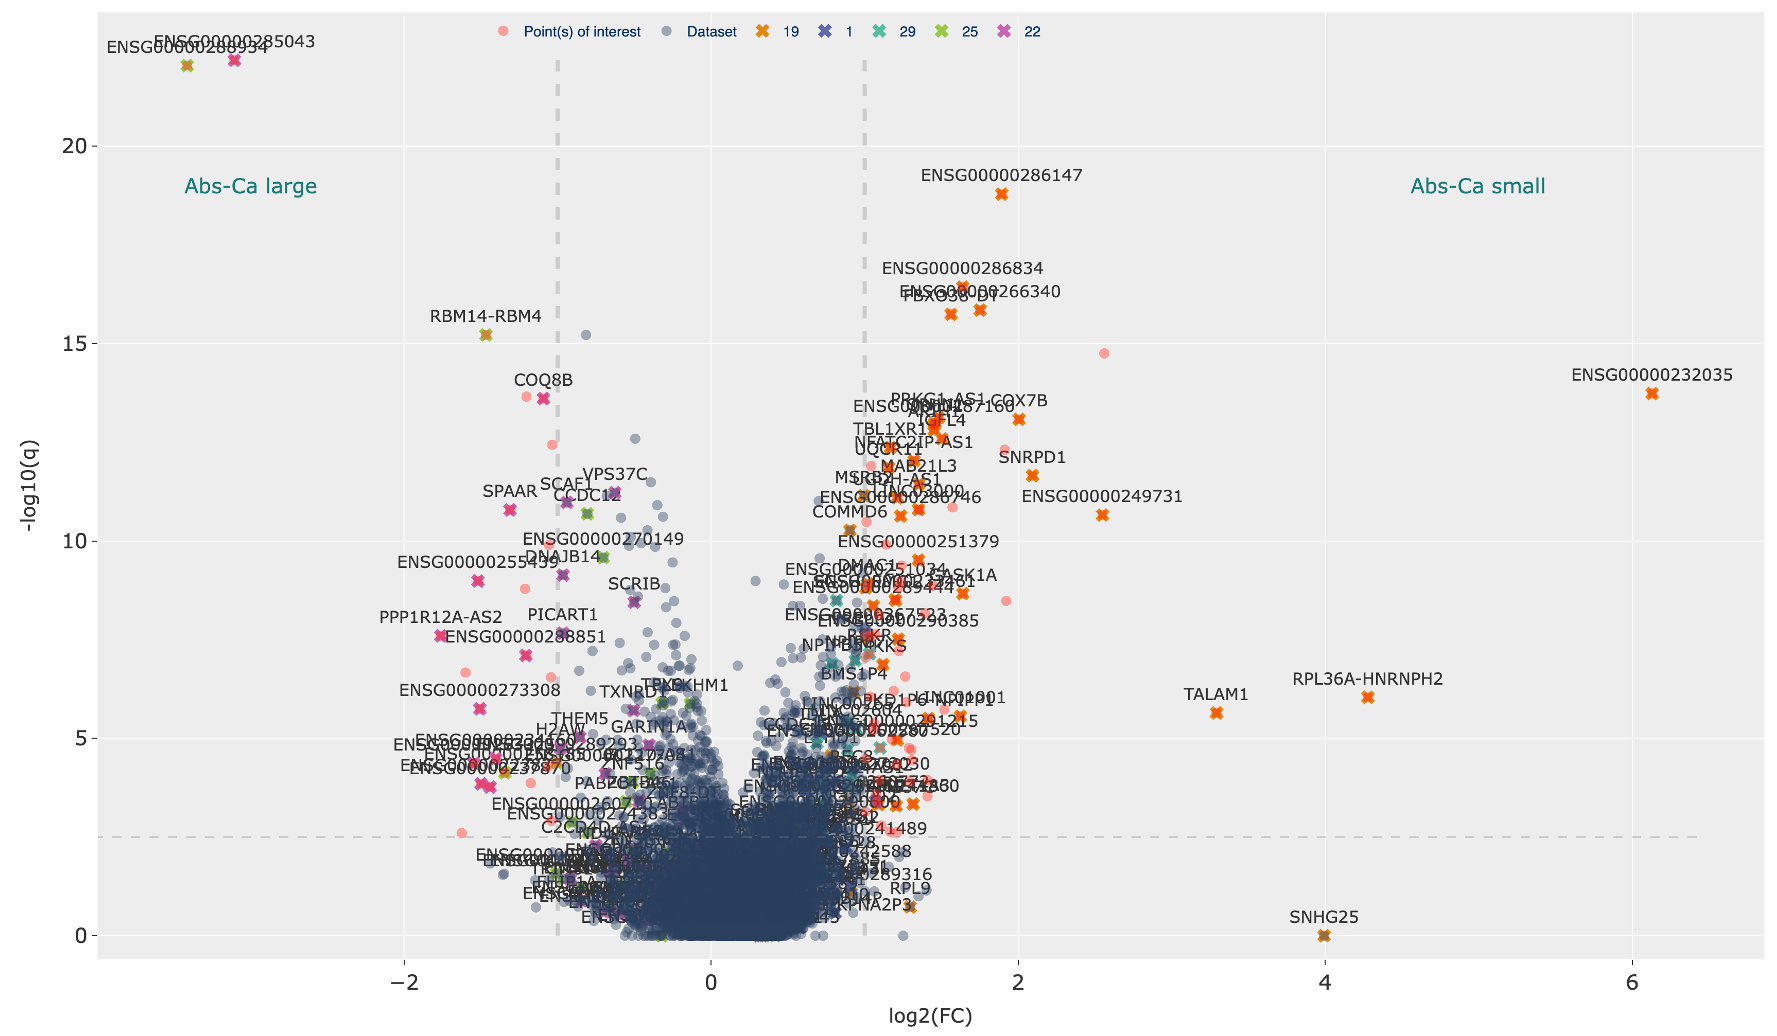
\includegraphics[width=1.0\textwidth,height=1.0\textheight,keepaspectratio]{Sections/Network_II/resources/non_tum/diff_split_dea.png}
    \caption{This is an annotated version of the Volcano plot in \cref{fig:N_II:diff_split} used for explanation purposes.}
    \label{fig:lit:dea_eg}
\end{figure}



% Pi 
\subsubsection{Pi plot} \label{s:lit:pi}

% Introduce to pi
The volcano plots are a great tool to understand the gene expression differences between two groups but are limited to two groups. To account for that \citet{Xiao2014-zn} introduced a new metric, pi-values (or $\pi$), which combines both the significance and the gene expression difference in one value using \cref{eq:lit:pi_val}. The $q-value$ represents the significance of the expression difference (from sleuth), and the $FC$ denotes the fold-change between the two compared groups. 

\begin{equation} \label{eq:lit:pi_val}
    pi = - log_{10}(q_{val}) * log_{2}(FC)
\end{equation} 

% Describe the comparison
By compressing the \acrshort{dea} results into one score enables 4 subtypes comparison, two on each of the axis of a scatter plot as seen in \cref{fig:lit:pi_eg}. The X-axis holds the pi values of the DEA between the P0 (group I) on the negative and Abs-Ca (group II) on the positive side. The  negative side y-values denote the genes specific to UD while the positive for Abs-Ca. As in the case with the Volcano plots, the scale of the axis is important and denotes the strength in the difference between the compared groups. This is highlighted by difference in shape by the coloured rectangles which are all within $+/-5\%$ of the axes and are a visual cue for the genes that are very close to the axis.

% Talk about the quadrant
As indicated by coloured rectangles, in \cref{fig:lit:pi_eg}, the closer to the axis a point is the more specific to that group is. The values between the coloured rectangles are part of a quadrant, starting from the right corner marked by Roman numbers (I, II, III, IV) represents the specific between two groups. In the case of \cref{fig:lit:pi_eg}, the first quadrant holds the genes that are specific to the Abs-Ca in the comparison with P0 (X) and with UD (Y). In quadrant II, the genes specific to the Abs-Ca over P0 and UD with respect to Abs-Ca. Quadrant III to both UD \& P0, and quadrant IV to P0 \& Abs-Ca.

% Quadrants
The figure from \cref{fig:lit:pi_eg} has three distinct groups, where Abs-Ca, an in-vitro tissue differentiated protocol, is compared on the X-axis against the P0 (\textbf{fresh sample analysed}) and on the Y-axis against the UD, an in-vitro tissue undifferentiated protocol. In this particular example, quadrant I holds the genes that are specific to the Abs-Ca group, giving a good characterisation of this particular tissue differentiated samples. The other quadrants represents the genes that are specific to the other two groups in the relation with Abs-Ca.

The pi-plots were extensively used in the project starting with the analysis of the MIBC groups from \cref{s:cs:bio_interp}, to the subtypes founds using a subset of \acrlong{tf} in \cref{s:N_I:sel_pruning} and the clusters derived with the latest version of the network approach in \cref{s:N_II:dea_rwd}.

\begin{figure}[!htb]    
    \centering
    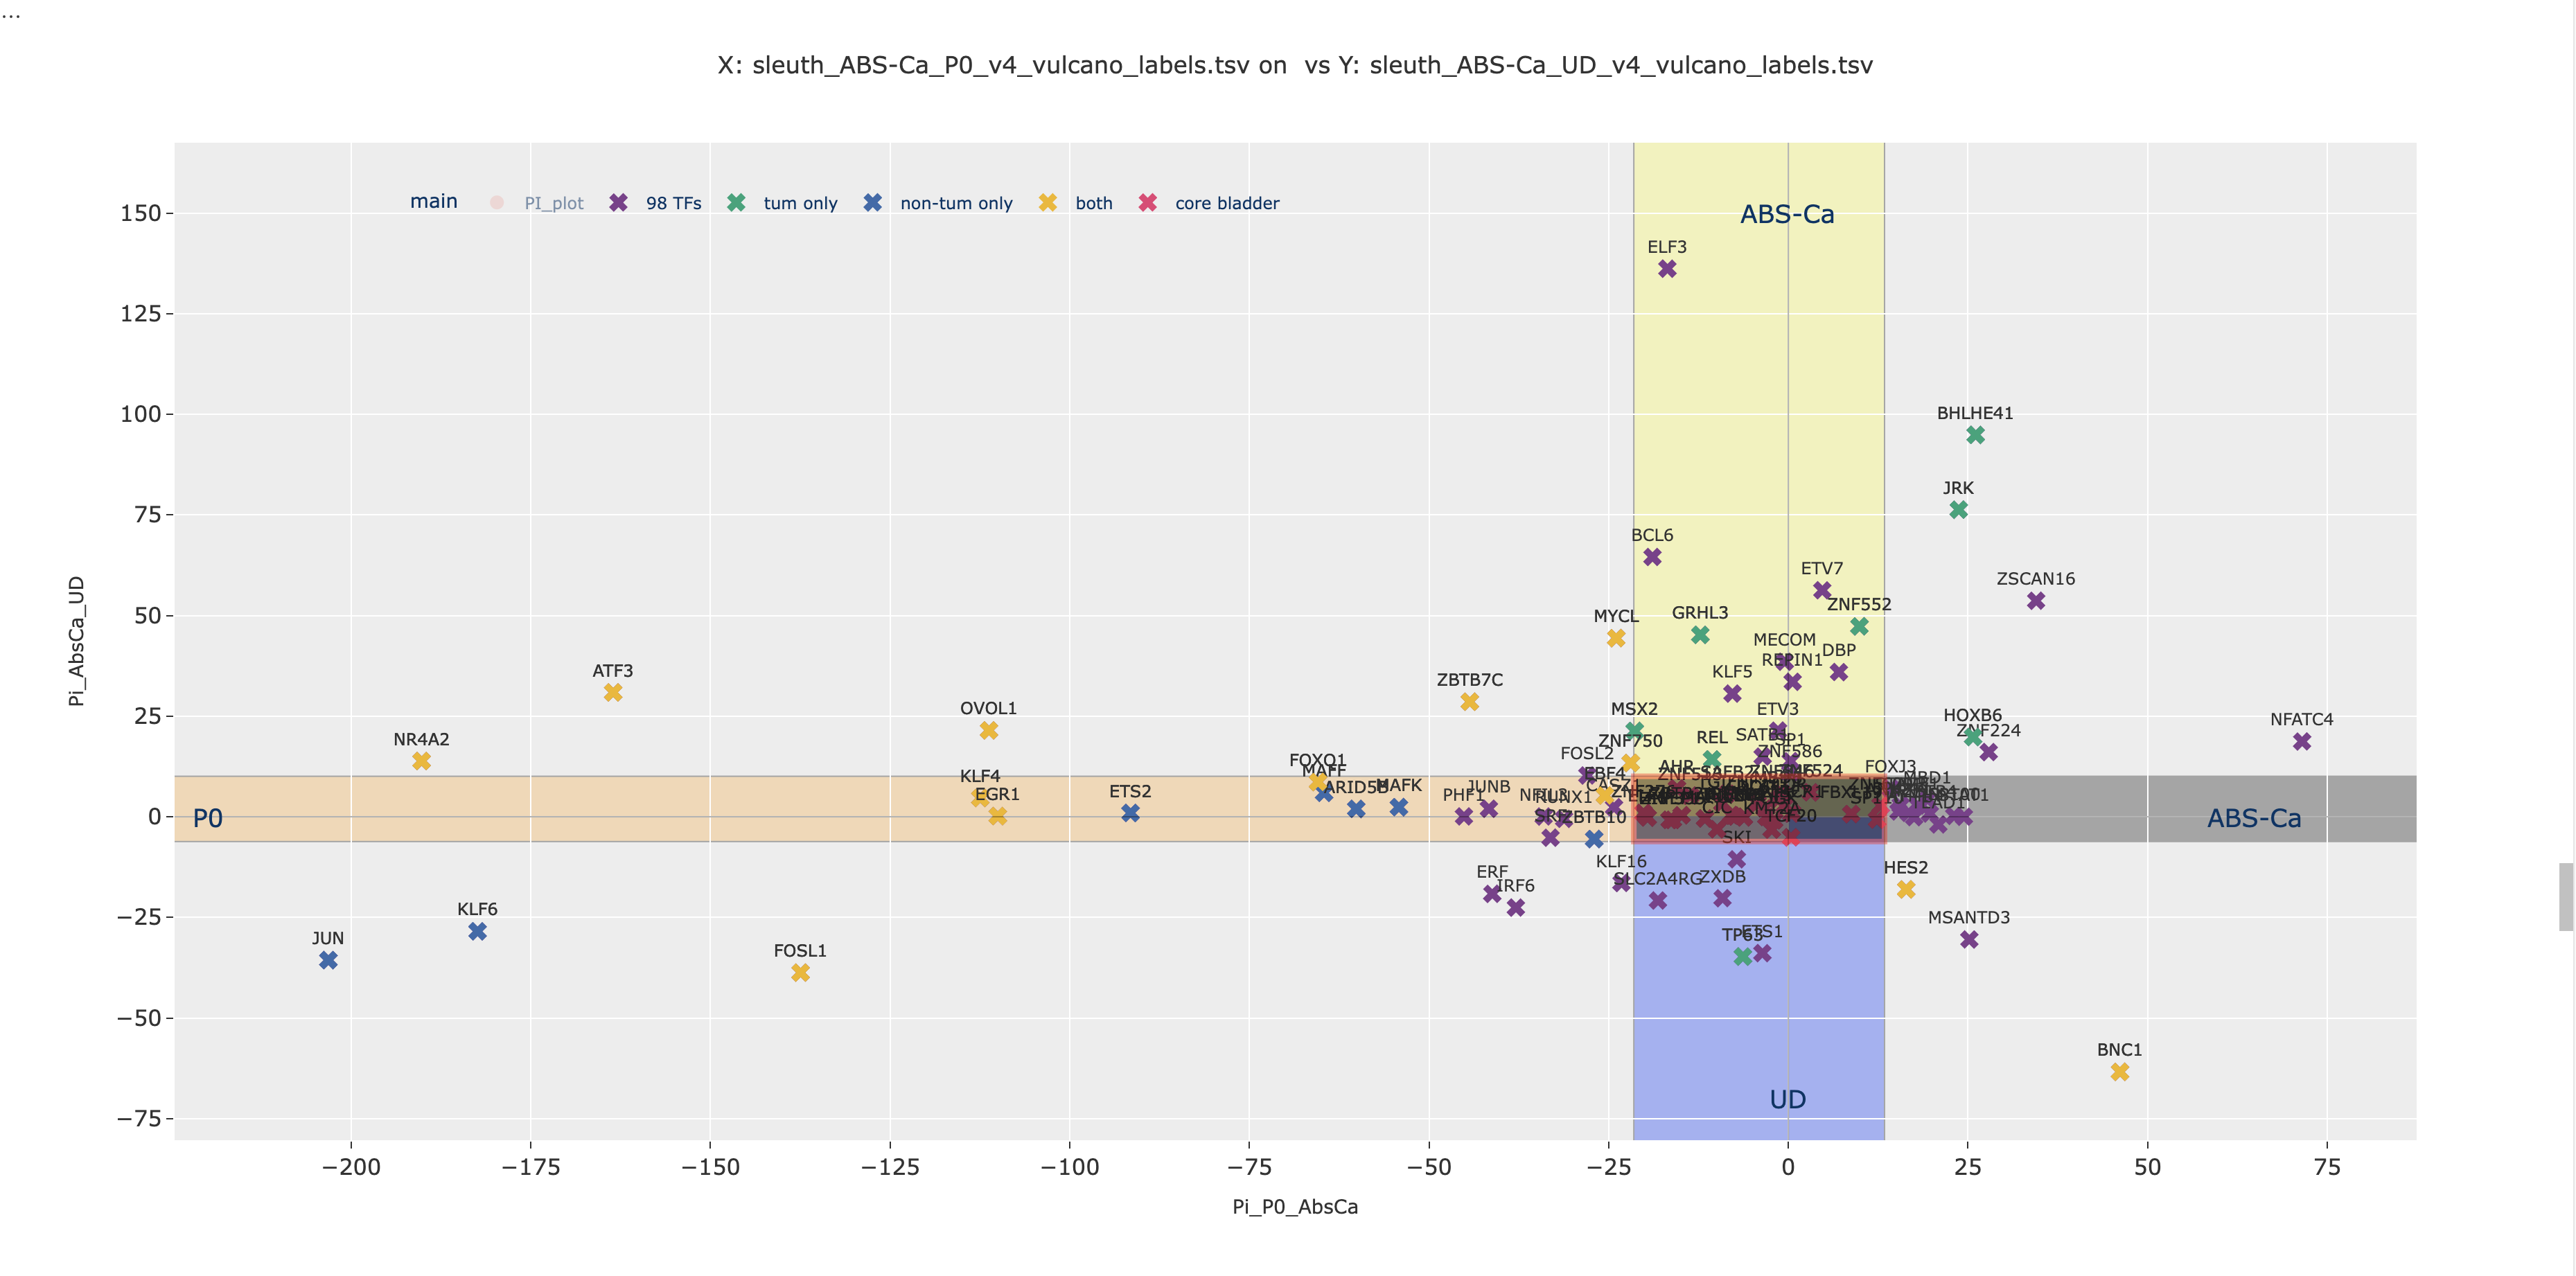
\includegraphics[width=1.0\textwidth,height=1.0\textheight,keepaspectratio]{Sections/Network_I/Resources/selective_pruning/sel_tfs_pi_all_var_rect.png}
    \caption{This is an annotated version of the Pi plot in \cref{fig:N_I:pi_sel_tfs_var} which is used to explain this type of figure.}
    \label{fig:lit:pi_eg}
\end{figure}

% GSEA
\subsubsection{Gene Set Enrichment Analysis} \label{s:lit:gsea}

% Introduction to GSEA
The volcano and pi plots introduced earlier are tools to identify genes specific to different groups, which are then used to perform \acrfull{gsea} using the GSEApy package by \citet{Fang2023-ec} and the REACTOME database\cite{Milacic2024-yt} \footnote{The reactome version \textit{c2.cp.reactome.v2023.2.Hs.symbols }was used in this project}.

% How GSEA works
GSEA works by ranking all genes in your dataset according to a predefined metric (such as expression level or statistical significance) and then assessing whether the members of a given gene set (e.g., from the REACTOME database) are randomly distributed throughout the ranked list or primarily found at the top or bottom. If many of the high-ranked genes correspond to the top genes in a REACTOME pathway, it indicates positive enrichment of that pathway. Conversely, if many lower-ranked genes match the top genes in a REACTOME pathway, it suggests that the pathway is depleted in the given context.

% Ranking system
In the pi-plot from \cref{fig:lit:pi_eg}, Quadrant I represents genes specific to the Abs-Ca group. To determine whether any of these genes are enriched in a REACTOME pathway, they must first be ranked. The blue cross, referred to as the 'Ref point,' represents the referential point, which consists of the maximum value on the X-axis (the most significantly expressed gene in comparison with P0) and the maximum on the Y-axis (the most significantly expressed gene in comparison with Abs-Ca). This point thus represents the 'most significantly expressed' coordinates across the two comparisons. The distances of all other points from this referential marker are computed, and the genes are then ranked. 

The GSEA was used to complement the Pi and Volcano plots in the second results chapters, \cref{s:N_I:sel_pruning}, where the subtypes were derived using a subset of \acrlong{tf}.

\begin{figure}[!htb]
    \centering
    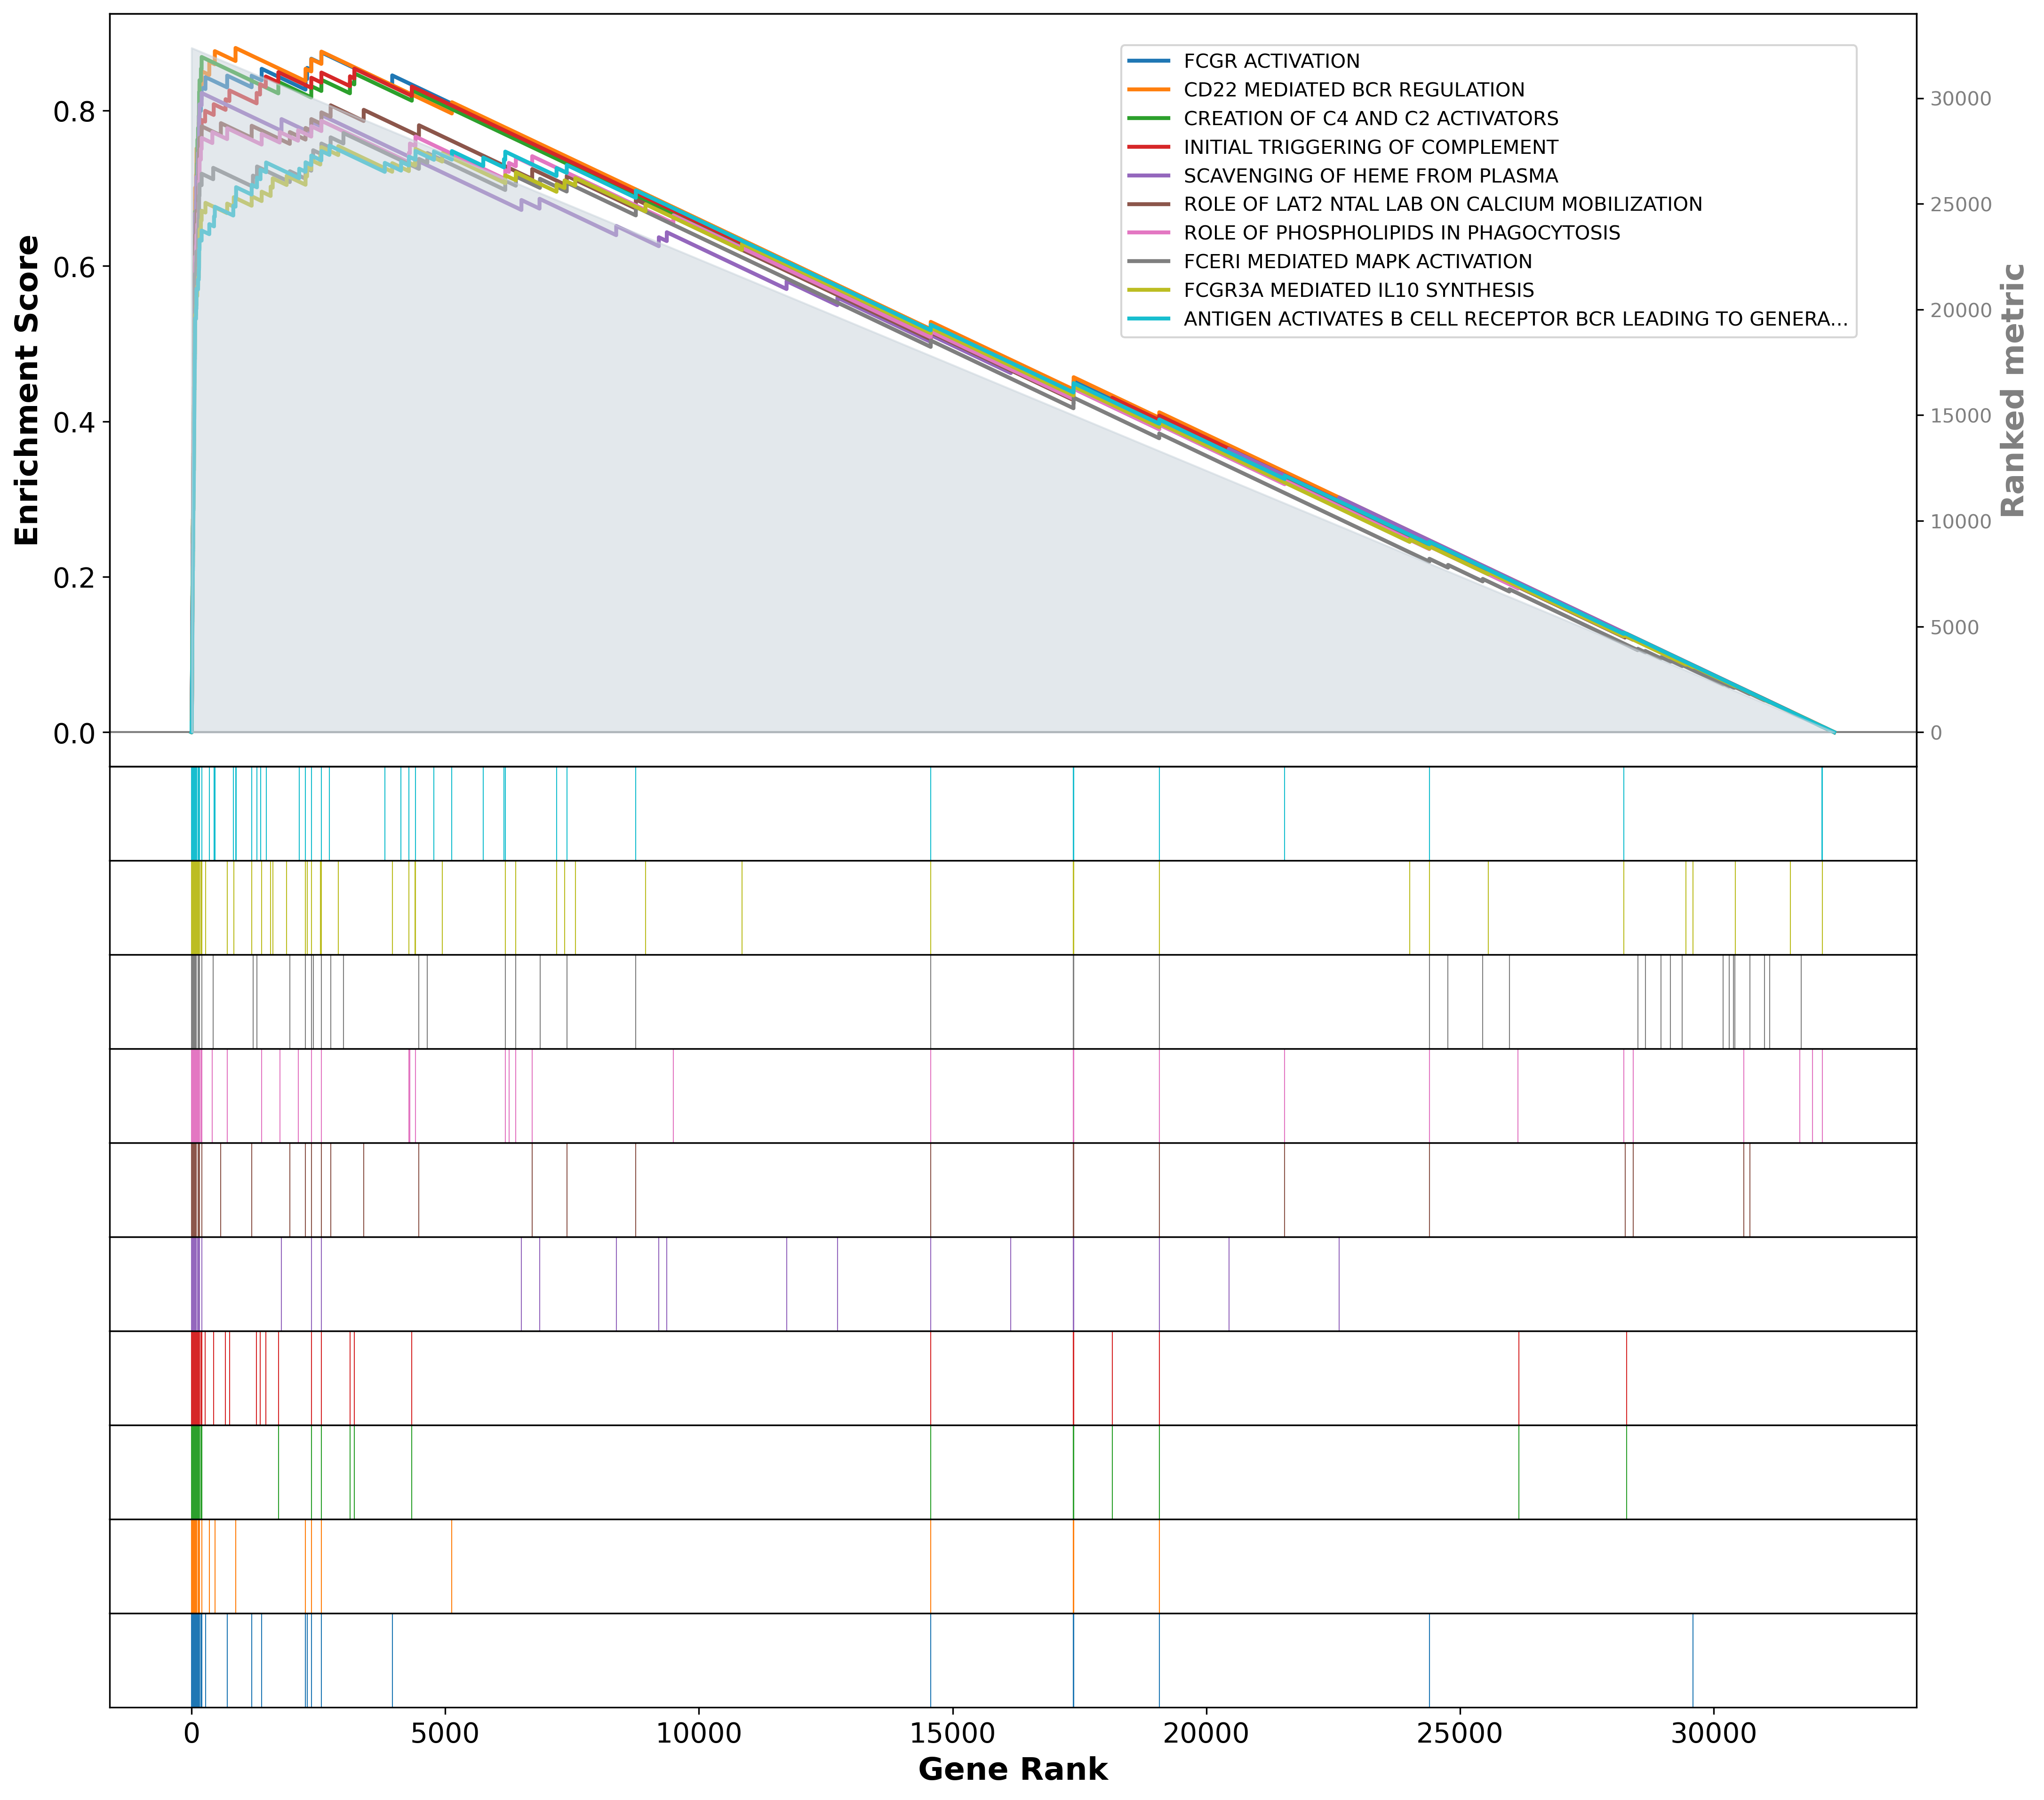
\includegraphics[width=0.8\textwidth, keepaspectratio]{Sections/ClusteringAnalysis/Resources/discussion/other_groups/lumInf_reactome_10_top.png}
        \caption{Top 10 GSEA results on the Reactome database.}
    \caption{Enrichment for the analysis in \cref{fig:cs:lumInf} used in the background chapter to showcase the \acrshort{gsea} . The group studied is the Luminal Infiltrated (LumInf) in quadrant III.}
    \label{fig:lit:gsea_eg}
\end{figure}

% Introduce the plot
The ranking system orders the genes in the pi-plot according to their expression difference and statistical significance. The ordered genes are then inputted to the GSEApy software which searches for pathways in the REACTOME database, producing a figure like \cref{fig:lit:gsea_eg}. \textbf{Note}, the GSEA in this case is run for the Luminal infiltrated group using the pi plot from \cref{s:cs:lumInf_interp} rather then the Abs-Ca group presented earlier in \cref{fig:lit:pi_eg}; this is because the GSEA did not return any significant enrichment scores for the Abs-Ca group.

% Describe the plot
The enrichment plot in \cref{fig:lit:gsea_eg} consists of two figures that share the same X-axis, which represents the gene ranking in ascending order, with the lowest-ranked gene closest to the referential point. The top figure plots the enrichment score (left Y-axis) of the pathways identified, while the bottom figure indicates the positions of the matched genes in the rank. The enrichment plot highlights the top 10 pathways with the highest enrichment scores, all of which have a significance level below 0.05. It is worth noting that the pathway names are abbreviated and trimmed (the "REACTOME" prefix removed) to fit the legend.

% Interpret the plot
The interpretation of enrichment analysis is performed by considering the collection of pathways identified rather than focusing on individual pathways. This is because genes can have different functions across various pathways, making it challenging to isolate a single pathway. For example, in \cref{fig:lit:gsea_eg}, multiple pathways are involved in immune-related functions, such as \textit{"FCCR Activation"}, \textit{"CD22 Mediated BCR Regulation"}, and \textit{"Antigen Activates B Cell Receptor..."}. Overall, the \acrshort{gsea} confirms the immune characteristics of the Luminal Infiltrated group, as identified in the clustering analysis in \cref{s:clustering_analysis}.

\subsection{Survival Analysis} \label{s:lit:survival}

% Introduce the plot
This project employs Kaplan-Meier survival analysis \citep{Kaplan1958-iy} to estimate the survival prognosis of patients in different MIBC groups. The metadata from \acrlong{tcga} and the lifelines package \citet{Davidson-Pilon2019-fu} are used to compute the survival statistics, as shown in the plot in \cref{fig:lit:surival_eg}.

% Present the figure
\Cref{fig:lit:surival_eg} represents the Kaplan-Meier analysis of the MIBC groups identified using the selective edge pruning method described in \cref{s:N_I:sel_pruning}. The Y-axis shows the probability of survival over time (in months), which is displayed on the X-axis for a period of five years. Each marker represents an observation of a patient's survival information, and the p-value is computed using a multivariate log-rank test, which allows for the determination of the significance of survival differences between more than two groups.

% Interpret the plot
The plot in \cref{fig:lit:surival_eg} indicates that patients in group 5 have the lowest survival prognosis, while those in group 13 have a better prognosis. The Kaplan-Meier survival plot is a valuable tool for assessing the significance of the new groups. In this case, all but 15\% of the patients in group 5 are deceased after 20 months, highlighting the potential impact of understanding this group on improving outcomes for bladder cancer patients.

The Kaplan-Meier survival analysis was used extensively throughout the project, beginning with the cluster analysis in \cref{s:clustering_analysis}, as shown in \cref{fig:cs:basal_survival,fig:cs:overview_survival}, followed by the selective edge pruning work in \cref{s:N_I:sel_pruning}, as illustrated in \cref{fig:N_I:sel_tfs_survival}, and finally in assessing the prognosis of the MIBC subtypes using the most advanced network configuration in \cref{s:N_II}, as presented in \cref{fig:N_II:survival_K_7}.


\begin{figure}[!htb]
    \centering
    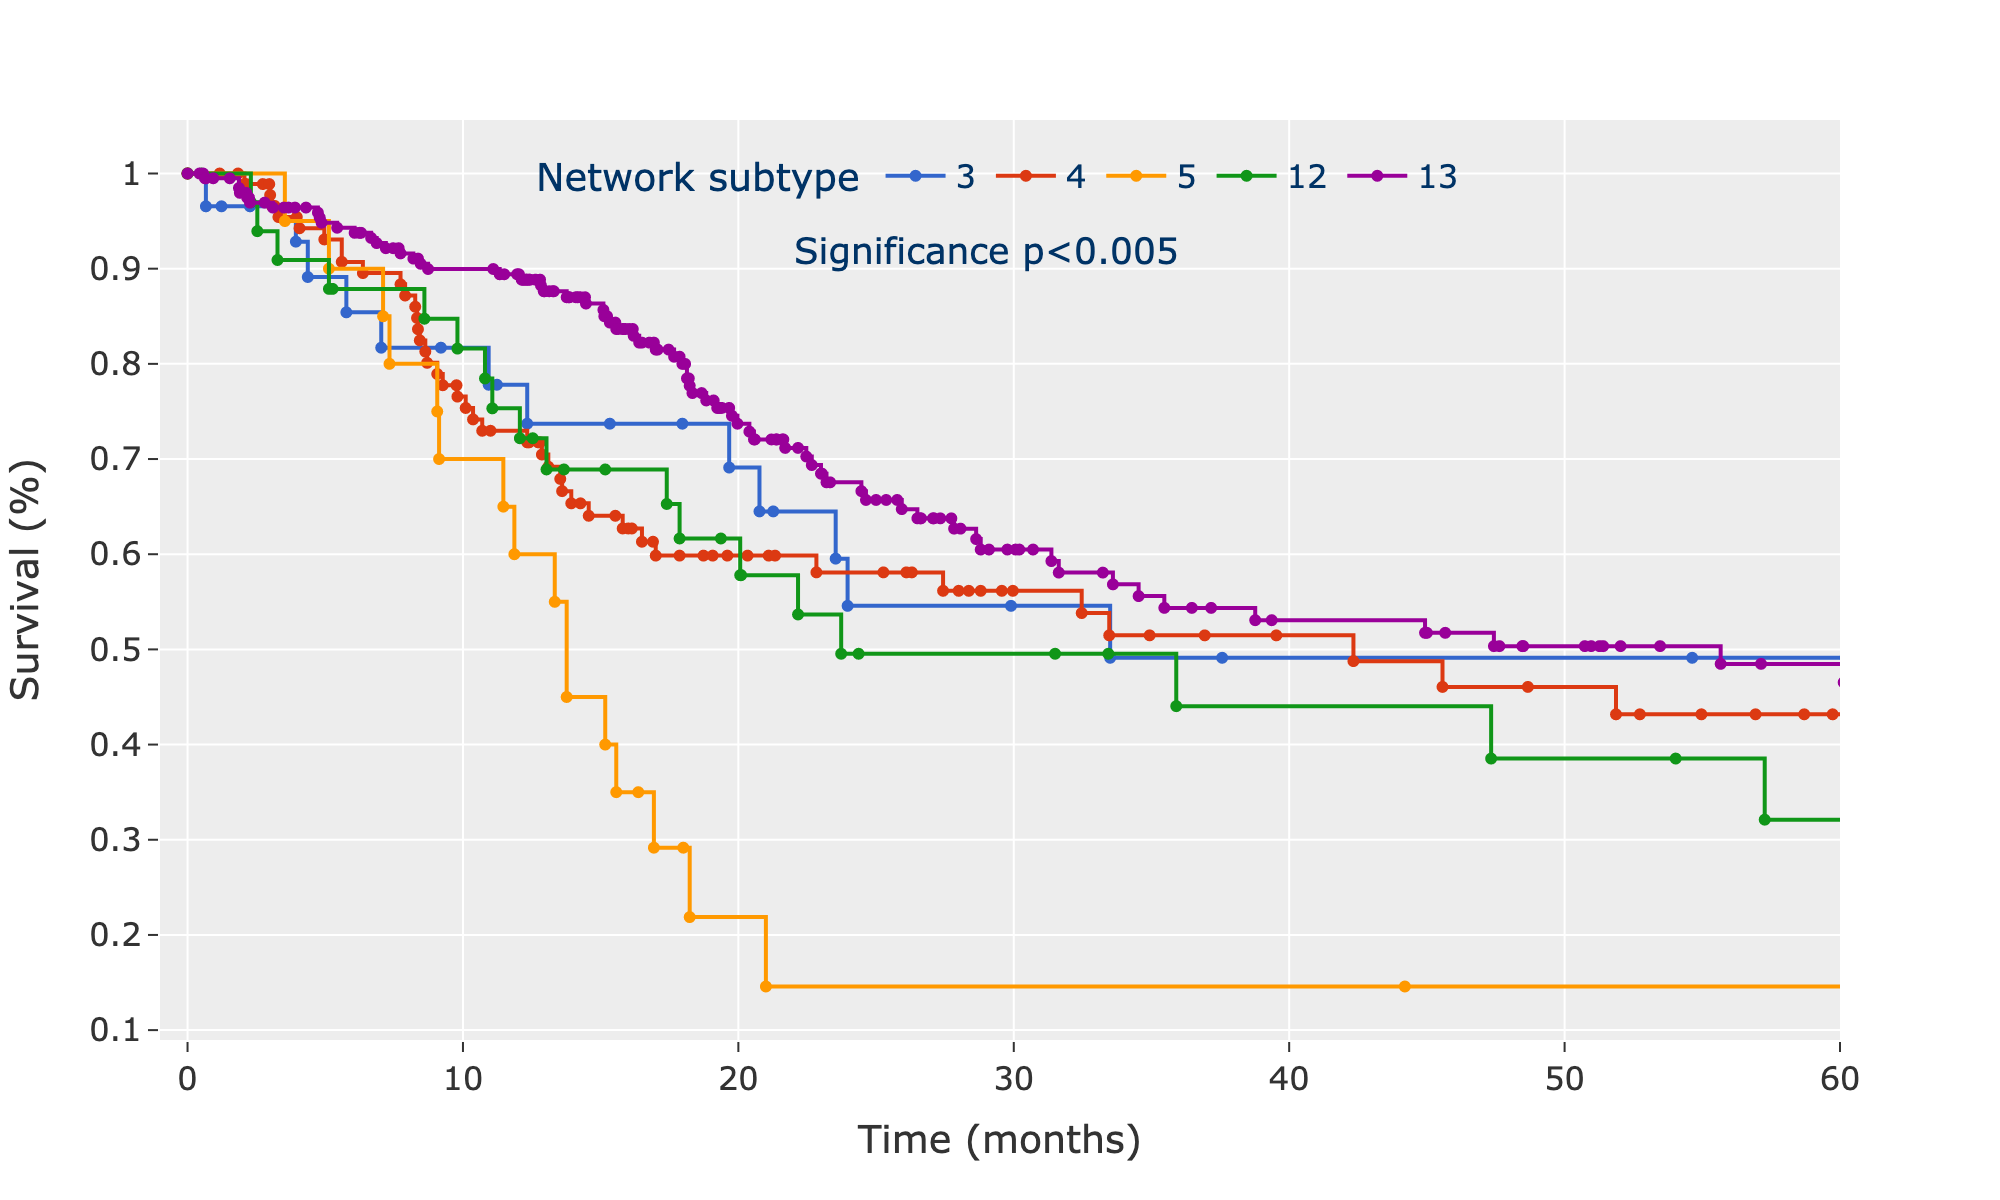
\includegraphics[width=1.0\textwidth,height=1.0\textheight,keepaspectratio]
    {Sections/Network_I/Resources/selective_pruning/survival_sel_tfs_cs.png}
    \caption{Kaplan-Meier survival analysis of the MIBC groups identified using the 98 TFs from \cref{s:N_I:sel_pruning}.}
    \label{fig:lit:surival_eg}
\end{figure}
